%\documentclass[]{beamer}
\documentclass[handout]{beamer}
% ***************************************************************
% for handout, change only this...
%   \documentclass[twocolumn]{article}
%   \usepackage{beamerarticle}
%   \setlength{\textwidth}{7.5in}
%   \setlength{\textheight}{9.8in}
%   \setlength{\topmargin}{-1in}  
%   \setlength{\oddsidemargin}{-.52in}  
%   \setlength{\evensidemargin}{-.52in}  

%\usepackage{beamerprosper}
%\usetheme{Warsaw}
%\usecolortheme{orchid}

\usepackage{graphicx}
\usepackage{amsmath,amssymb,array,comment,eucal}
\newcommand{\e}{\mathbf{e}}
\renewcommand{\P}{\mathbf{P}}
\newcommand{\F}{\mathbf{F}}
\newcommand{\R}{\textsf{R}}
\newcommand{\mat}[1] {\mathbf{#1}}
%\newcommand{\ind}{\mathrel{\mathop{\sim}\limits^{\mathit{ind}}}}
%\newcommand{\iid}{\mathrel{\mathop{\sim}\limits^{\mathit{iid}}}}
\newcommand{\E}{\textsf{E}}
\newcommand{\SE}{\textsf{SE}}
\newcommand{\SSE}{\textsf{SSE}}
\newcommand{\RSS}{\textsf{RSS}}
\newcommand{\FSS}{\textsf{FSS}}
\renewcommand{\SS}{\textsf{SS}}
\newcommand{\MSE}{\textsf{MSE}}
\newcommand{\SSR}{\textsf{SSR}}
\newcommand{\Be}{\textsf{Beta}}
\newcommand{\St}{\textsf{St}}
%\newcommand{\C}{\textsf{C}}
\newcommand{\GDP}{\textsf{GDP}}
\newcommand{\NcSt}{\textsf{NcSt}}
\newcommand{\Bin}{\textsf{Bin}}
\newcommand{\NB}{\textsf{NegBin}}
\renewcommand{\NG}{\textsf{NG}}
\newcommand{\N}{\textsf{N}}
\newcommand{\Ber}{\textsf{Ber}}
\newcommand{\Poi}{\text{Poi}}
\newcommand{\Gam}{\textsf{Gamma}}
\newcommand{\BB}{\textsf{BB}}
\newcommand{\Gm}{\textsf{G}}
\newcommand{\Un}{\textsf{Unif}}
\newcommand{\Ex}{\textsf{Exp}}
\newcommand{\DE}{\textsf{DE}}
\newcommand{\tr}{\textsf{tr}}
\newcommand{\cF}{{\cal{F}}}
\newcommand{\cL}{{\cal{L}}}
\newcommand{\cI}{{\cal{I}}}
\newcommand{\cB}{{\cal{B}}}
\newcommand{\cP}{{\cal{P}}}
\newcommand{\bbR}{\mathbb{R}}
\newcommand{\bbN}{\mathbb{N}}
\newcommand{\pperp}{\mathrel{{\rlap{$\,\perp$}\perp\,\,}}}
\newcommand{\OFP}{(\Omega,\cF, \P)}
\newcommand{\eps}{\boldsymbol{\epsilon}}
\newcommand{\1}{\mathbf{1}_n}
\newcommand{\gap}{\vspace{8mm}}
\newcommand{\ind}{\mathrel{\mathop{\sim}\limits^{\rm ind}}}
\newcommand{\simiid}{\ensuremath{\mathrel{\mathop{\sim}\limits^{\rm
iid}}}}
\newcommand{\eqindis}{\ensuremath{\mathrel{\mathop{=}\limits^{\rm D}}}}
\newcommand{\iid}{\textit{i.i.d.}}
\newcommand{\SSZ}{S_{zz}}
\newcommand{\SZW}{S_{zw}}
\newcommand{\Var}{\textsf{Var}}
\newcommand{\corr}{\textsf{corr}}
\newcommand{\diag}{\textsf{diag}}
\newcommand{\var}{\textsf{var}}
\newcommand{\Cov}{\textsf{Cov}}
\newcommand{\Sam}{{\cal S}}
\def\H{\mathbf{H}}
\newcommand{\I}{\mathbf{I}}
\newcommand{\Y}{\mathbf{Y}}
\newcommand{\tY}{\tilde{\mathbf{Y}}}
\newcommand{\Yhat}{\hat{\mathbf{Y}}}
\newcommand{\Yobs}{\mathbf{Y}_{{\cal S}}}
\newcommand{\barYobs}{\bar{Y}_{{\cal S}}}
\newcommand{\barYmiss}{\bar{Y}_{{\cal S}^c}}
\def\bv{\mathbf{b}}
\def\X{\mathbf{X}}
\def\tX{\tilde{\mathbf{X}}}
\def\x{\mathbf{x}}
\def\xbar{\bar{\mathbf{x}}}
\def\Xbar{\bar{\mathbf{X}}}
\def\Xg{\mathbf{X}_{\boldsymbol{\gamma}}}
\def\Ybar{\bar{\Y}}
\def\ybar{\bar{y}}
\def\y{\mathbf{y}}
\def\Yf{\mathbf{Y_f}}
\def\W{\mathbf{W}}
\def\L{\mathbf{L}}
\def\w{\mathbf{w}}
\def\U{\mathbf{U}}
\def\V{\mathbf{V}}
\def\Q{\mathbf{Q}}
\def\Z{\mathbf{Z}}
\def\z{\mathbf{z}}
\def\v{\mathbf{v}}
\def\u{\mathbf{u}}

\def\zero{\mathbf{0}}
\def\one{\mathbf{1}}
\newcommand{\taub}{\boldsymbol{\tau}}
\newcommand{\betav}{\boldsymbol{\beta}}
\newcommand{\alphav}{\boldsymbol{\alpha}}
\newcommand{\A}{\mathbf{A}}
\def\a{\mathbf{a}}
\def\K{\mathbf{K}}
\newcommand{\B}{\mathbf{B}}
\def\b{\boldsymbol{\beta}}
\def\bhat{\hat{\boldsymbol{\beta}}}
\def\btilde{\tilde{\boldsymbol{\beta}}}
\def\tb{\tilde{\boldsymbol{\beta}}}
\def\bg{\boldsymbol{\beta_\gamma}}
\def\bgnot{\boldsymbol{\beta_{(-\gamma)}}}
\def\mub{\boldsymbol{\mu}}
\def\tmub{\tilde{\boldsymbol{\mu}}}
\def\muhat{\hat{\boldsymbol{\mu}}}
\def\t{\boldsymbol{\theta}}
\def\tk{\boldsymbol{\theta}_k}
\def\tj{\boldsymbol{\theta}_j}
\def\Mk{\boldsymbol{{\cal M}}_k}
\def\M{\boldsymbol{{\cal M}}}
\def\Mj{\boldsymbol{{\cal M}}_j}
\def\Mi{\boldsymbol{{\cal M}}_i}
\def\Mg{{\boldsymbol{{\cal M}_\gamma}}}
\def\Mnull{\boldsymbol{{\cal M}}_{N}}
\def\gMPM{\boldsymbol{\gamma}_{\text{MPM}}}
\def\gHPM{\boldsymbol{\gamma}_{\text{HPM}}}
\def\Mfull{\boldsymbol{{\cal M}}_{F}}
\def\tg{\boldsymbol{\theta}_{\boldsymbol{\gamma}}}
\def\g{\boldsymbol{\gamma}}
\def\eg{\boldsymbol{\eta}_{\boldsymbol{\gamma}}}
\def\G{\mathbf{G}}
\def\cM{\cal M}
\def\D{\Delta}
\def \shat{{\hat{\sigma}}^2}
\def\uv{\mathbf{u}}
\def\l {\lambda}
\def\d{\delta}
\def\Sigmab{\boldsymbol{\Sigma}}
\def\Lambdab{\boldsymbol{\Lambda}}
\def\lambdab{\boldsymbol{\lambda}}
\def\Mg{{\cal M}_\gamma}
\def\S{{\cal{S}}}
\def\qg{p_{\boldsymbol{\gamma}}}
\def\pg{p_{\boldsymbol{\gamma}}}
\def\t{\boldsymbol{\theta}}  
\def\T{\boldsymbol{\Theta}}  
\title{Mixtures of Prior Distributions}

\author{Hoff Chapter 9, Liang et al 2007, Hoeting et al (1999), Clyde \&
 George (2004)} 
\date{\today}
%\Logo(-1.9,7.3){\includegraphics[width=.5in]{../eps/duke}}
% Optional: text to put in the bottom of each slide.
% By default, the title of the talk will be placed there.
%\slideCaption{\textit{October 28, 2005 }}

\begin{document}
% make the title slide
\maketitle


\begin{frame}
  \frametitle{Bartlett's Paradox}
 The Bayes factor for comparing $\Mg$ to the null
model:
$$
 BF(\Mg : \M_0) =    (1 + g)^{(n - 1 - \pg)/2} (1 + g(1 - R_{\g}^2))^{-(n-1)/2}
$$
\pause 
For $g \to \infty$, the  $BF \to 0$ for fixed $n$ and $R_{\g}^2$
\end{frame}


\begin{frame}
  \frametitle{Information Paradox}
  
The Bayes factor for comparing $\Mg$ to the null
model:
$$
 BF(\Mg : \M_0) =    (1 + g)^{(n - 1 - \pg)/2} (1 + g(1 - R^2))^{-(n-1)/2}
$$
\pause
\begin{itemize}
\item Let $g$ be a fixed constant and take $n$ fixed. \pause
\item Let $F = \frac{R_{\g}^2/\pg}{(1 - R_{\g}^2)/(n - 1 - \pg)}$ \pause
\item As $R^2_{\g} \to 1$, $F \to \infty$ LR test would reject $\M_0$
  where $F$ is the usual $F$ statistic for  comparing model $\Mg$ to
  $\M_0$ \pause 
\item BF converges to a fixed constant $(1+g)^{-\pg/2}$  (does not go
  to infinity
\end{itemize}

``Information Inconsistency''  see Liang et al JASA 2008


\end{frame}
\begin{frame}
  \frametitle{Mixtures of $g$ priors \& Information consistency}
  
Need $BF \to \infty$ if $\R^2 \to 1$  $\Leftrightarrow$ $\E_g[(1 +
g)^{-\pg/2}]$ diverges  (proof in Liang et al)
\pause
\begin{itemize}
\item Zellner-Siow Cauchy prior \pause
\item hyper-g prior (Liang et al JASA 2008) 
$$p(g) = \frac{a-2}{2}(1 + g)^{-a/2}$$ or $g/(1+g) \sim Beta(1, (a-2)/2)$ 
need $2 < a \le 3$
\pause
\item Hyper-g/n  $(g/n)(1 + g/n) \sim (Beta(1, (a-2)/2)$ \pause
\item Jeffreys prior on $g$ corresponds to $a = 2$ (improper)
\item robust prior (Bayarrri et al Annals of Statistics 2012 \pause
\item Intrinsic prior (Womack et al  JASA 2015)
\end{itemize}

 All have prior tails for $\b$  that behave like a Cauchy distribution
 and (the latter 4) marginal  likelihoods that can be computed using special hypergeometric
 functions   ($_2F_1$, Appell $F_1$)
\end{frame}

\begin{frame}\frametitle{Desiderata - Bayarri et al 2012 AoS}
  \begin{itemize}
  \item Proper priors on non-common coefficients \pause
  \item If LR overwhelmingly rejects a model, Bayesian should also
    reject \pause
  \item Selection Consistency: large samples probability of the true model goes
    to one. \pause
  \item Intrinsic prior consistency (prior converges to a fixed proper
    prior as $n \to \infty$  \pause
  \item Invariance  (invariance under scale/location changes of
    data/model leads to $p(\beta_0, \phi) \propto 1/\phi$); other
    group invariance, rotation invariance.  \pause
\item predictive matching:  predictive distributions match under
  minimal sample sizes so that $BF = 1$
  \end{itemize}
  
\end{frame}
\section{Mortality}
\begin{frame}[fragile]
\frametitle{Mortality \& Pollution}
  \begin{itemize}
  \item Data from Statistical Sleuth 12.17 \pause 
  \item 60 cities \pause 
\item response Mortality \pause 
\item measures of HC, NOX, SO2 \pause 
\item Is pollution associated with mortality after adjusting for other
  socio-economic and meteorological factors? \pause 
\item 15 predictor variables implies $2^{15} = 32,768$ possible models
  \pause 
\item Use Zellner-Siow Cauchy prior  $1/g \sim  G(1/2, n/2)$
  \end{itemize}
\begin{verbatim}
mort.bma = bas.lm(MORTALITY ~ ., data=mortality,
                  prior="ZS-null", 
                  alpha=60,  n.models=2^15, 
                  update=100, initprobs="eplogp")
\end{verbatim}
\end{frame}

\begin{frame}\frametitle{Posterior Distributions}
  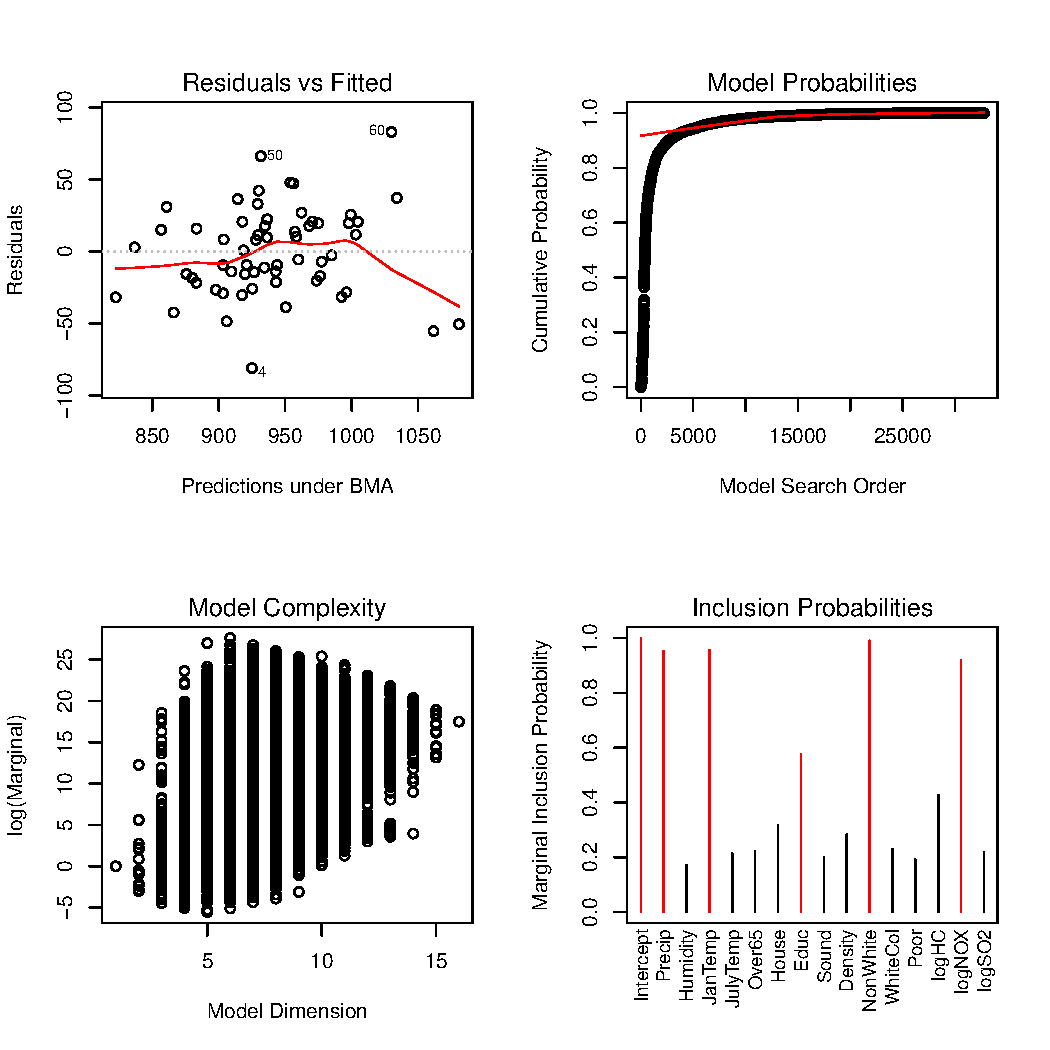
\includegraphics[height=3.5in]{mort-sum}
\end{frame}



\begin{frame}[fragile]
\frametitle{Posterior Probabilities}
  \begin{itemize}
  \item What is the probability that there is no pollution effect? \pause 
\item Sum posterior model probabilities over all models that include
  no pollution variables \pause 
\begin{verbatim}
> which.mat = list2matrix.which(mort.bma,1:(2^15))
> poll.in = (which.mat[, 14:16] %*% rep(1, 3)) > 0
> sum(poll.in * mort.bma$postprob)
[1] 0.9889641
\end{verbatim}\pause 
\item Posterior probability  no effect is $0.011$ \pause 
\item Posterior Odds that there is an effect  $(1 - .011)/(.011) = 89.$ \pause 
\item Prior Odds $7 = (1 - .5^3)/.5^3$ \pause 
\item Bayes Factor for a pollution effect $ 89.9/7 = 12.8$ \pause 
\item Bayes Factor for NOX based on marginal inclusion probability
  $0.917/(1 - 0.917) = 11.0$ \pause  
\item Marginal inclusion probability for logHC =  0.427144 ($BF=.745$)
\item Marginal inclusion probability for logSO2 = 0.218978 ($BF=.280$)
\end{itemize}
Bayes Factors are not additive! 
\end{frame}
\begin{frame}\frametitle{Model Space}
  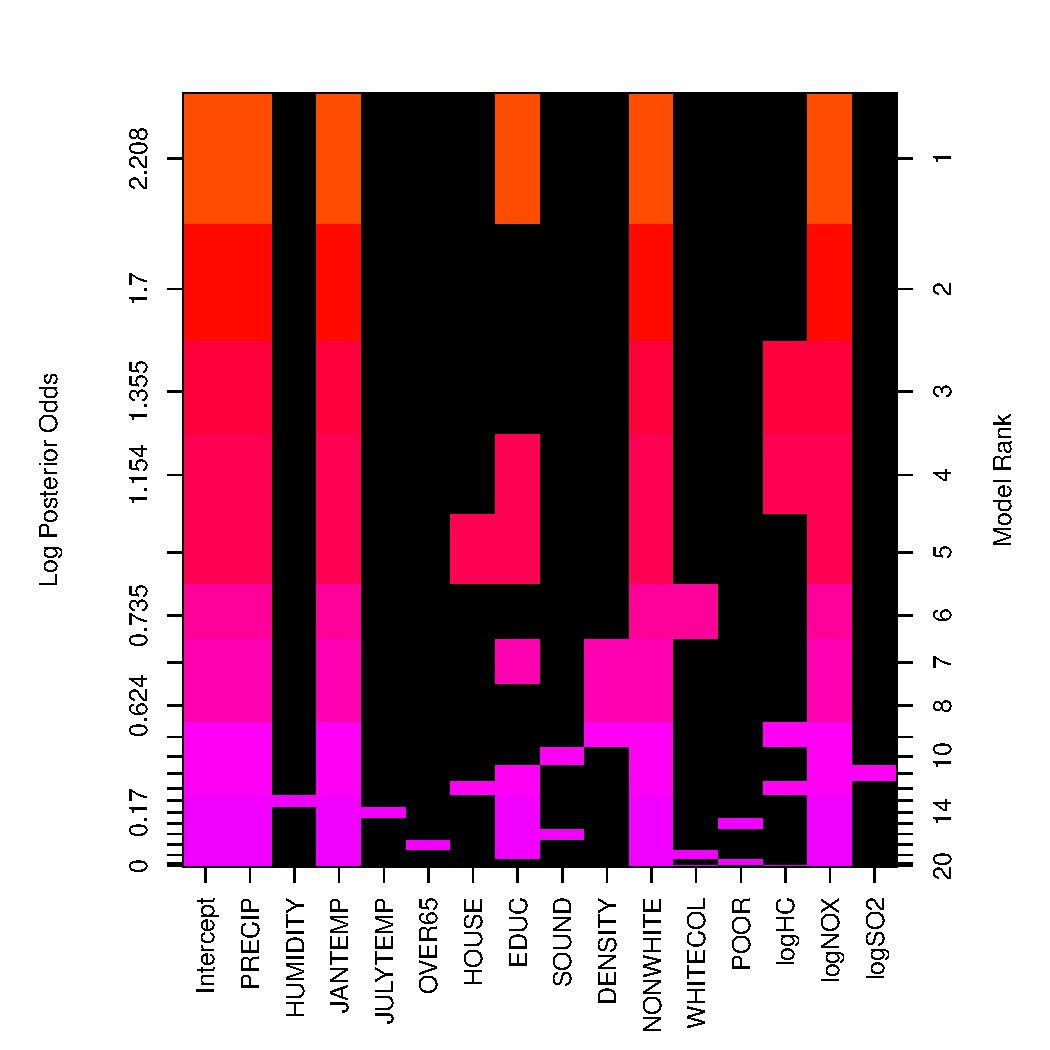
\includegraphics[height=3.5in]{mort-image}
\end{frame}
\begin{frame}\frametitle{Coefficients}
  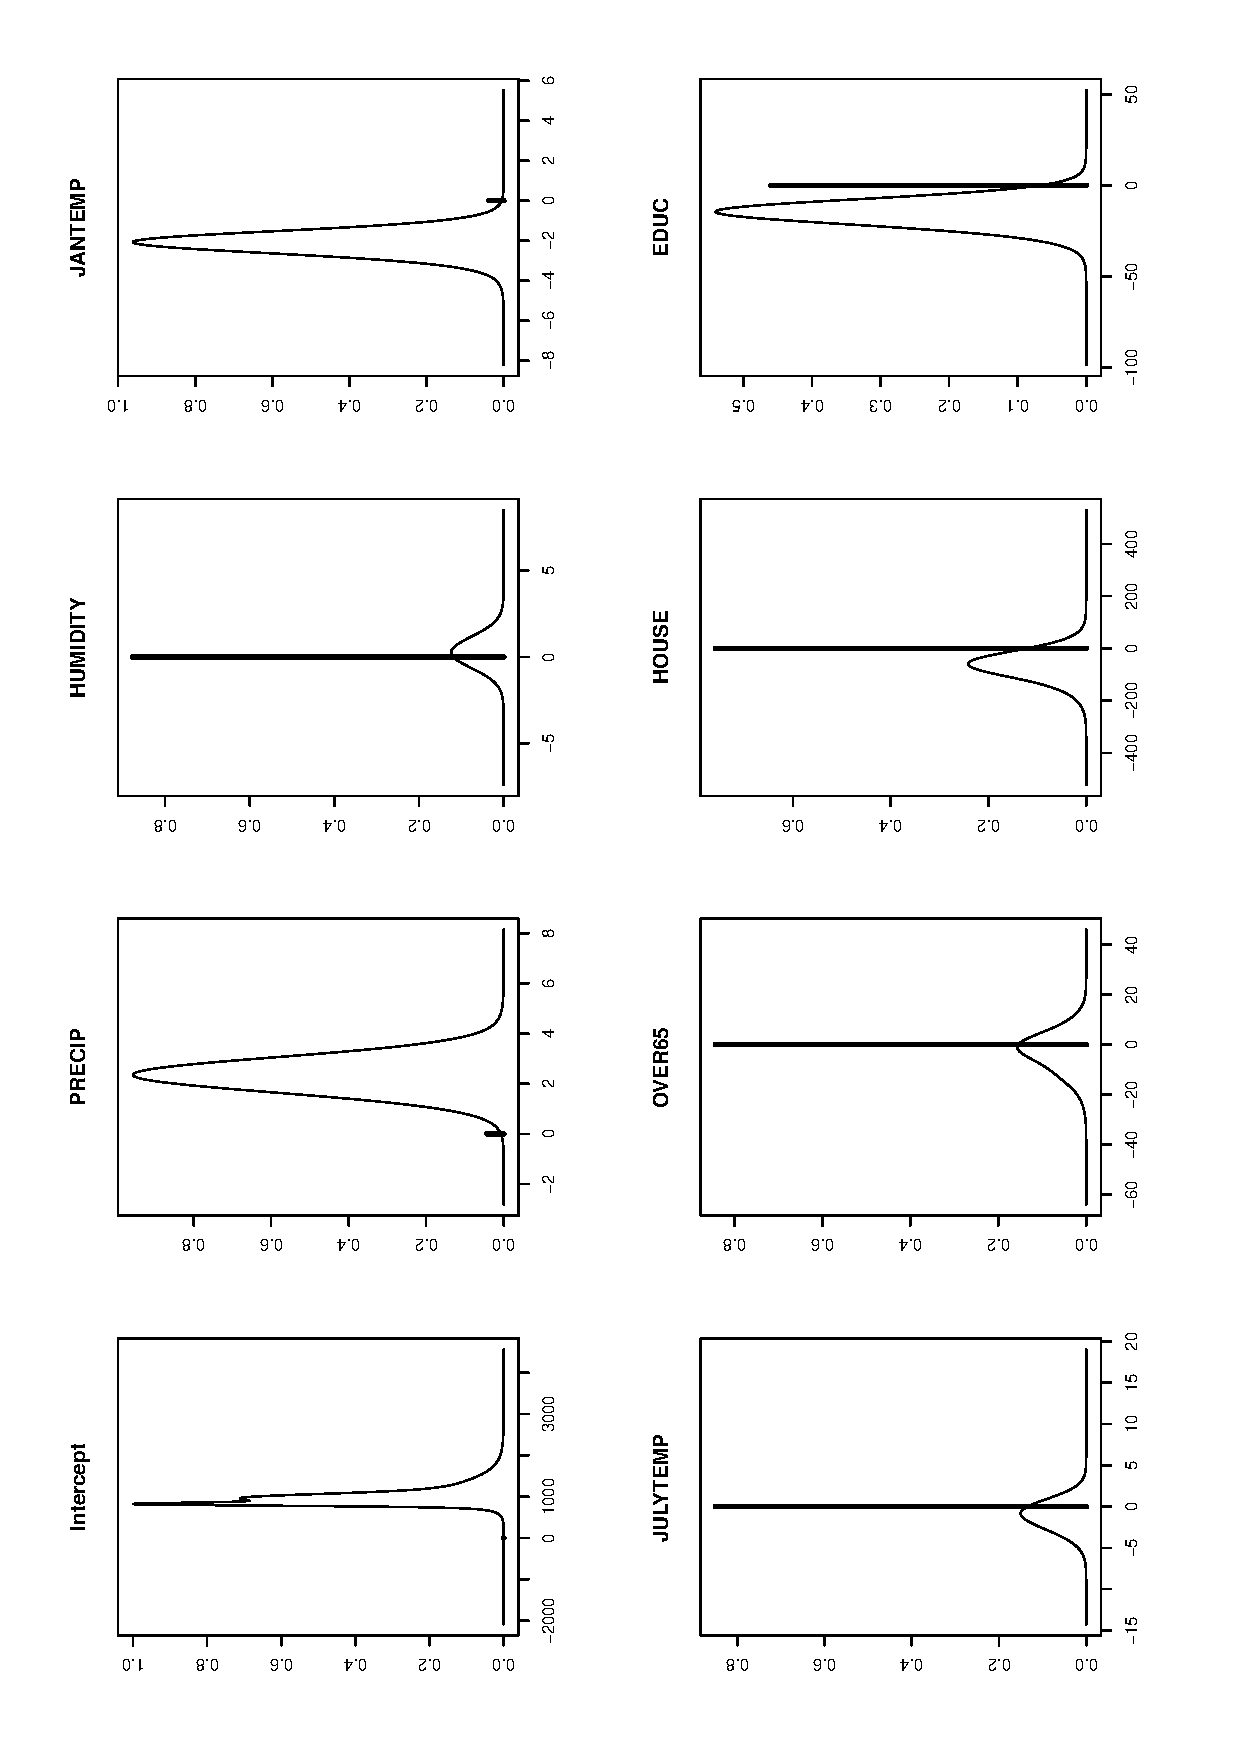
\includegraphics[height=3.5in]{mort-beta1}
\end{frame}

\begin{frame}\frametitle{Coefficients}
  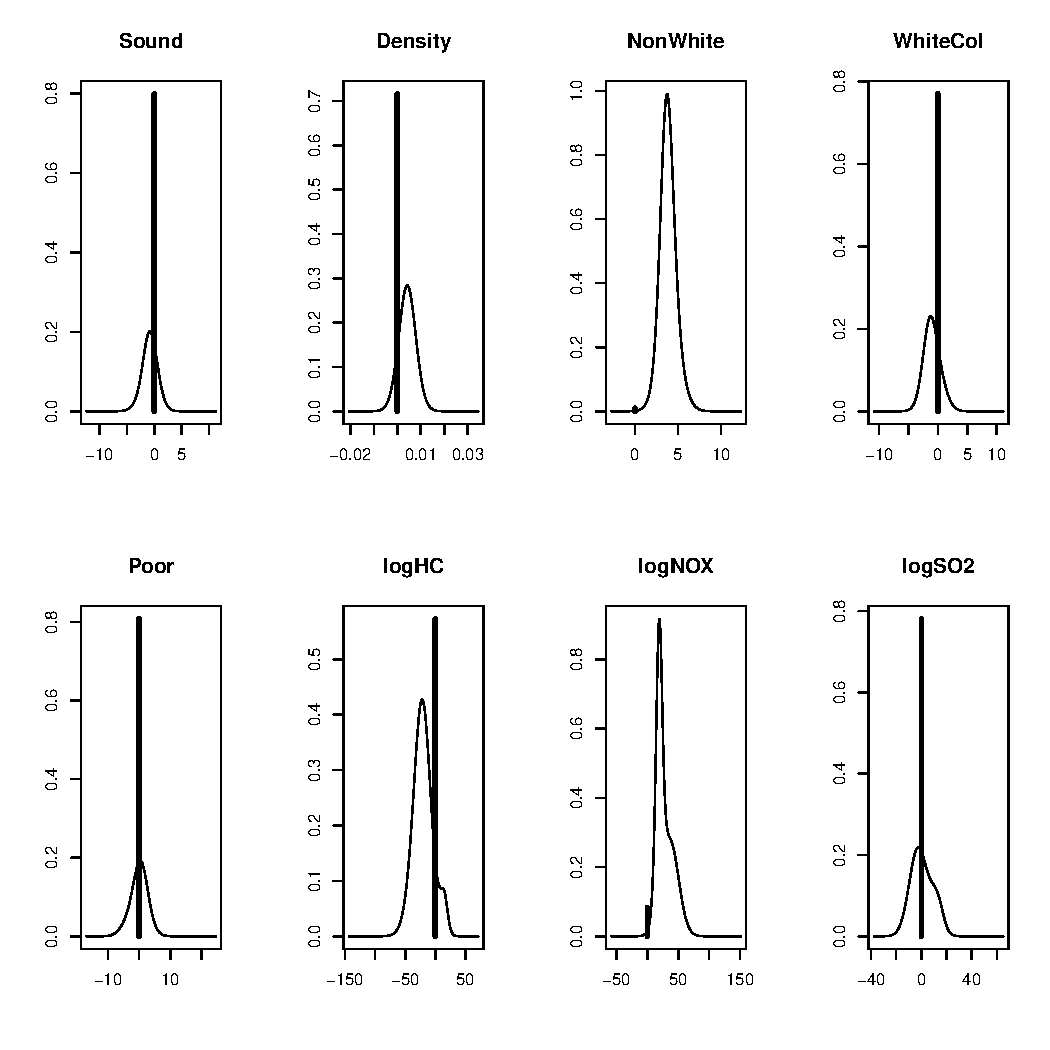
\includegraphics[height=3.5in]{mort-beta2}
\end{frame}

\begin{frame}
  \frametitle{Effect Estimation}
  \begin{itemize}
  \item  Coefficients in each model are adjusted for other variables
    in the model
\item OLS:  leave out a predictor with a non-zero coefficient then
  estimates are biased!
\item Model Selection in the presence of high correlation, may leave
  out "redundant" variables; 
\item improved MSE for prediction (Bias-variance tradeoff)
\item Bayes is biased anyway so should we care?
\item What is meaning of $\sum_{\g} \beta_{j \g} \gamma_j P(\Mg \mid \Y)$
  \end{itemize}
  With confounding, should not use plain BMA.  Need to change prior?

\end{frame}



\begin{frame}\frametitle{ Other Problems}


  \begin{itemize}
  \item Computational \pause 
  if $p > 35$  enumeration is difficult \pause 
  \begin{itemize}
  \item Gibbs sampler or Random-Walk algorithm on $\g$ \pause 
  \item poor convergence/mixing with high correlations \pause 
  \item Metropolis Hastings algorithms more flexibility
    (method="MCMC") \pause 
  \item "Stochastic Search" (no guarantee samples represent posterior)
    \pause 
\item Variational, EM, etc to find modal model \pause
  \item in BMA all variables are included, but coefficients are 
   shrunk to 0; alternative is to use Shrinkage methods \pause 
  \item Models with Non-estimable parameters?   (use generalized inverse)
  \end{itemize}
\item Prior Choice: Choice of prior distributions on $\b$ and on $\g$
  \pause 
\end{itemize}

\bigskip Model averaging versus Model Selection  -- what are objectives?


\end{frame}

\begin{frame}\frametitle{BAS Algorithm - Clyde, Ghosh, Littman - JCGS}
  Sampling w/out Replacing
\end{frame}

\end{document}
